\begin{figure}[H]
	\center
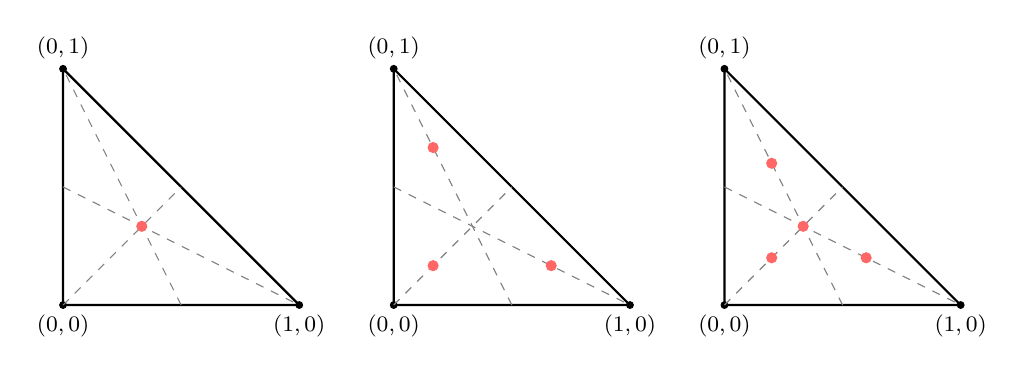
\begin{tikzpicture}[scale=3]
		
		\def \xone{0};
		\def \yone{0};		
		% first rectangle
		\coordinate (A) at (\xone,\yone);
		
        \draw[thick] (A) -- ++(0,1) -- ++(1,-1)--cycle;
        \filldraw (A)         circle (0.4pt);
        \filldraw (A) ++(1,0) circle (0.4pt);
        \filldraw (A) ++(0,1) circle (0.4pt);
        \fill[black,font=\footnotesize] (A)         node[below] {$(0,0)$}
                                        (A) ++(0,1) node[above] {$(0,1)$}
                                        (A) ++(1,0) node[below] {$(1,0)$};
        \draw[dashed,gray] (A) ++(0,1/2) -- ++(1,-1/2);
        \draw[dashed,gray] (A) -- ++(1/2,1/2);
        \draw[dashed,gray] (A) ++(1/2,0) -- ++(-1/2,1);
        
        \filldraw[red!60] (A)++(1/3, 1/3) circle (0.6pt);
        
        
        % second rectangle
        \coordinate (A1) at (\xone + 1.4,\yone);
        
        \draw[thick] (A1) -- ++(0,1) -- ++(1,-1)--cycle;
        \filldraw (A1)         circle (0.4pt);
        \filldraw (A1) ++(1,0) circle (0.4pt);
        \filldraw (A1) ++(0,1) circle (0.4pt);
        \fill[black,font=\footnotesize] (A1)         node[below] {$(0,0)$}
								        (A1) ++(0,1) node[above] {$(0,1)$}
        								(A1) ++(1,0) node[below] {$(1,0)$};
        
        \draw[dashed,gray] (A1) ++(0,1/2) -- ++(1,-1/2);
        \draw[dashed,gray] (A1) -- ++(1/2,1/2);
        \draw[dashed,gray] (A1) ++(1/2,0) -- ++(-1/2,1);
        
        \filldraw[red!60] (A1)++(1/6, 1/6) circle (0.6pt);
        \filldraw[red!60] (A1)++(2/3, 1/6) circle (0.6pt);
        \filldraw[red!60] (A1)++(1/6, 2/3) circle (0.6pt);
        
        % third rectangle
        \coordinate (A2) at (\xone + 2.8,\yone);
        
        \draw[thick] (A2) -- ++(0,1) -- ++(1,-1)--cycle;
        \filldraw (A2)         circle (0.4pt);
        \filldraw (A2) ++(1,0) circle (0.4pt);
        \filldraw (A2) ++(0,1) circle (0.4pt);
        \fill[black,font=\footnotesize] (A2)         node[below] {$(0,0)$}
        								(A2) ++(0,1) node[above] {$(0,1)$}
 								        (A2) ++(1,0) node[below] {$(1,0)$};
        
        \draw[dashed,gray] (A2) ++(0,1/2) -- ++(1,-1/2);
        \draw[dashed,gray] (A2) -- ++(1/2,1/2);
        \draw[dashed,gray] (A2) ++(1/2,0) -- ++(-1/2,1);
        
        \filldraw[red!60] (A2)++(1/3, 1/3) circle (0.6pt);
        \filldraw[red!60] (A2)++(1/5, 3/5) circle (0.6pt);
        \filldraw[red!60] (A2)++(1/5, 1/5) circle (0.6pt);
        \filldraw[red!60] (A2)++(3/5, 1/5) circle (0.6pt);
\end{tikzpicture}

\caption{Visualisation of other nodes in $\hat{T}$ for $N_Q =1,3,4$ (order 1,2,3)}
\label{ch_quad__other_nodes_T_hat}
\end{figure}